\section{Outils de développement}

\subsection{Analyseur Logique Intégré}
L'environnement de développement Xilinx met à disposition une IP appelée IPA pour analyseur logique intégré (Integrated Logic Analyzer).
Cet outil peut être instancié dans le FPGA et permet de capturer les chronogrammes des signaux souhaités.
Il est parfaitement adapté pour le debug de l'interface AXI mais peut être connecté à tout autre point d'intérêt.
Une source d'horloge synchrone au design observé doit idéalement être connectée. \cite{ILA_doc}
Les données enregistrées pourront directement être visibles dans l'interface "Harware manager" de Vivado.
La figure \ref{fig:ILA} illustre un exemple d'utilisation de l'ILA en observation du bus AXI.
\begin{figure}[H]
    \centering
    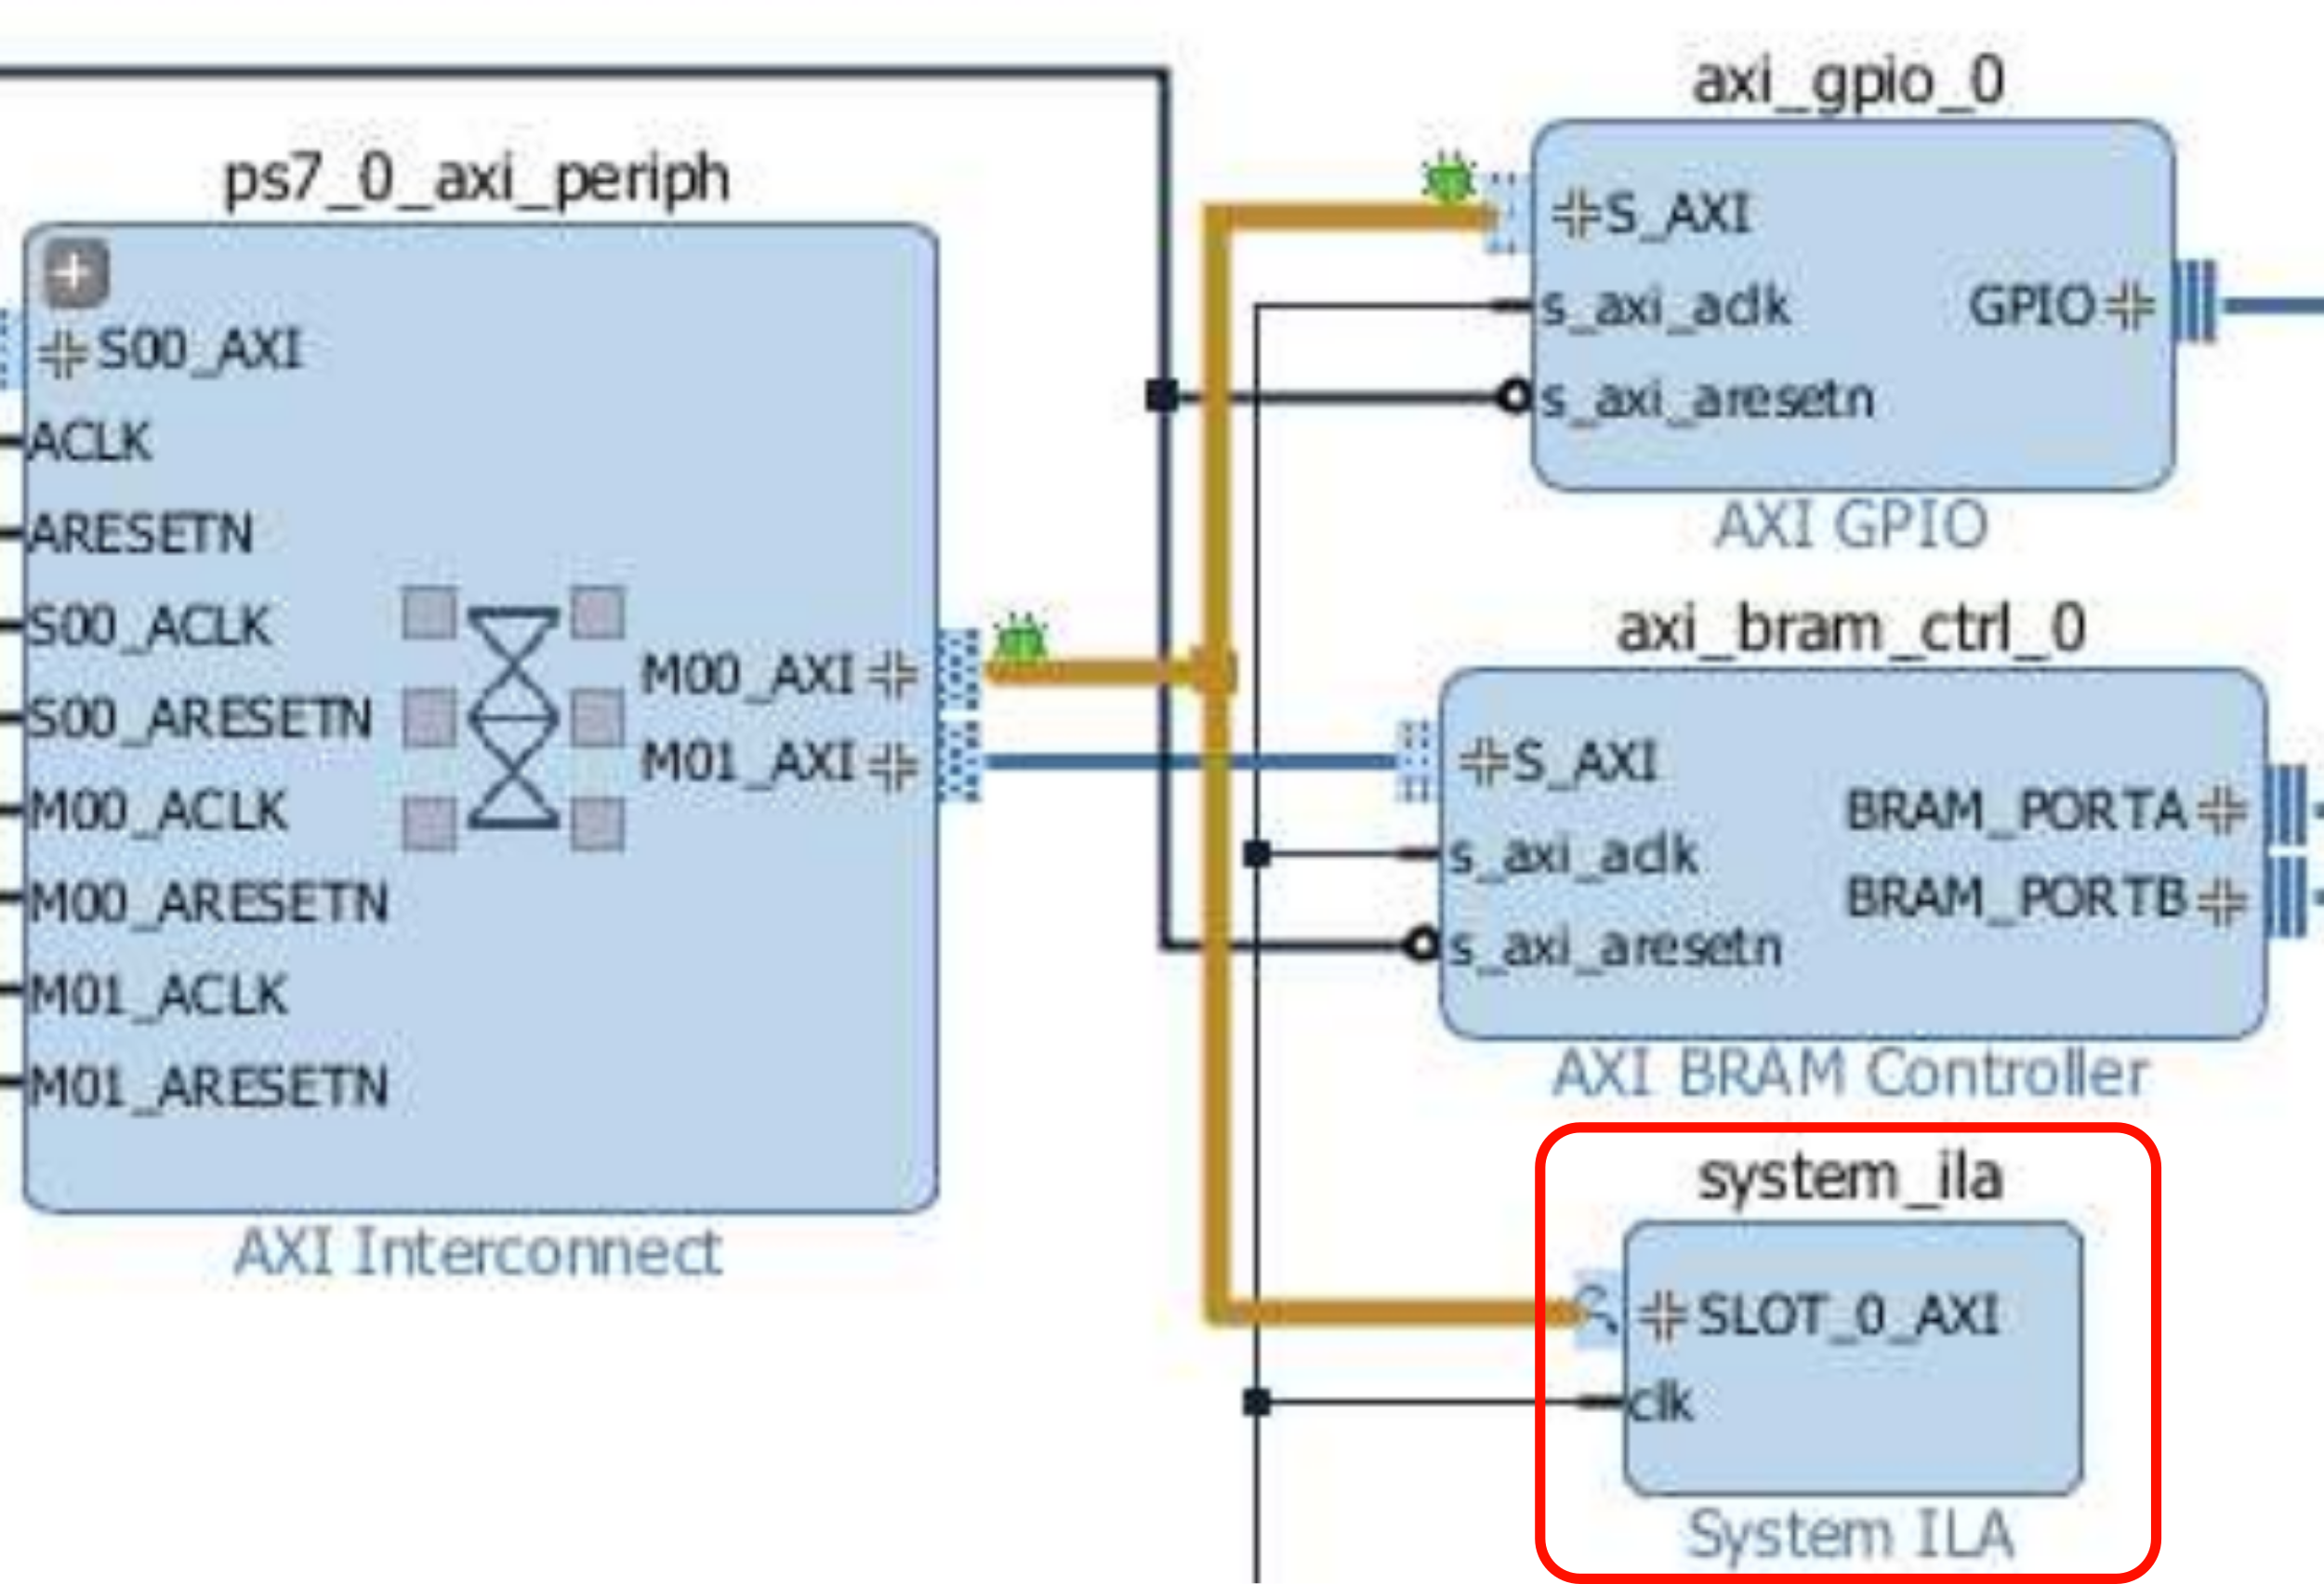
\includegraphics[width=0.6\linewidth]{ILA.png}
    \caption{Positionnement de l'IP ILA sur un bus AXI}
    \label{fig:ILA}
\end{figure}
% On montre que l'on métrise la consomation des ressources logiques
Les blocs logiques habituels sont utilisés pour implémenter la sonde d'échantillonnage et les triggers.
Les valeurs des signaux échantillonnées sont ensuite sauvegardé dans la RAM.
L'utilisation de l'ILA n'est possible qu'à condition d'avoir les ressources logiques nécessaires.
Il est probablement possible de faire varier sa surface d'occupation en déduisant le nombre de sondes et la complexité des réglages lors de l'instanciation.
N'ayant pas d'informations supplémentaires sur la taille du circuit à tester, nous feront l'hypothèse la plus optimiste pour laquelle aucun problème d'espace n'est rencontré.

\subsection{Débugueur logiciel}
%TODO
